% !TEX TS-program = pdflatexmk
% !BIB TS-program = bibtex

\documentclass[12pt, a4paper, twoside]{book}
\usepackage{import}
\subimport{../}{preamble}
\ExecuteBibliographyOptions{articletitle=false}
\standalonetrue
\onehalfspacing
\begin{document}

\begin{singlespace}
\color{white}
\chapter{Introduction}
\end{singlespace}

\AddToShipoutPictureBG*{
	\AtPageUpperLeft{
		\put(0,-235) {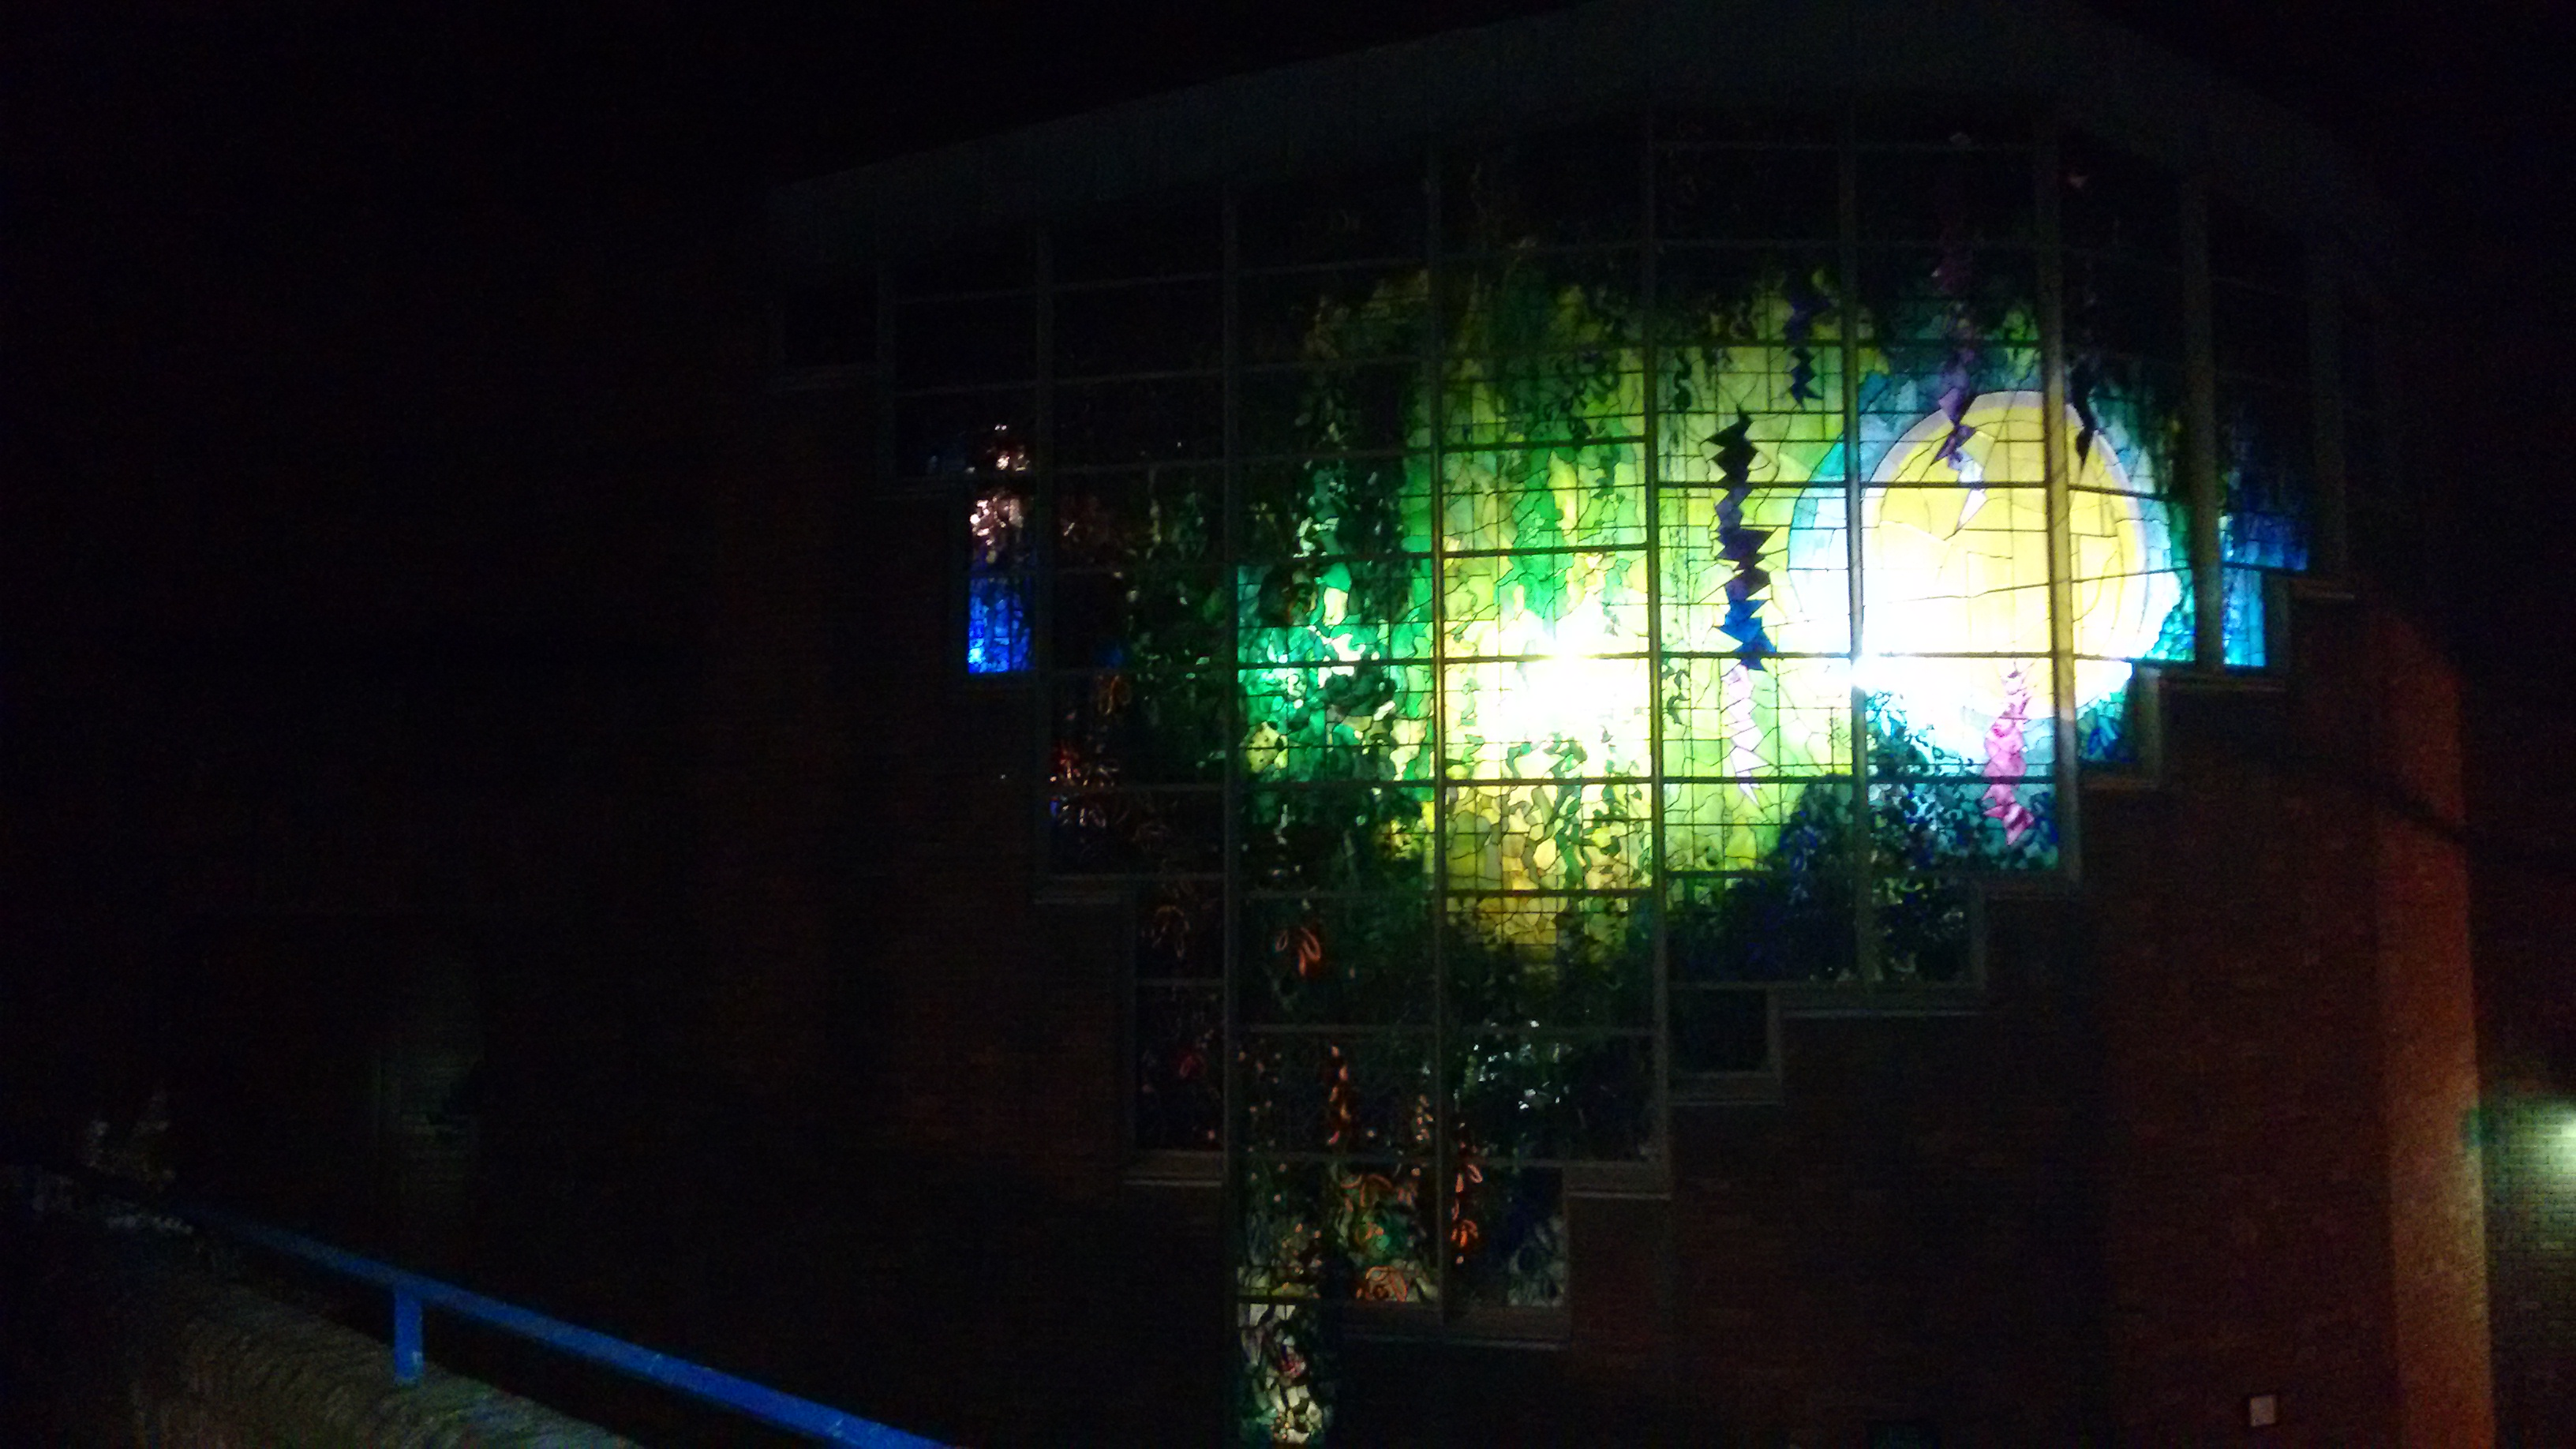
\includegraphics[width=\paperwidth, clip=true, trim=0 250 0 0]{figures/chapter_cover.jpg}}
		\put(280,-220) {\begin{minipage}{0.65\textwidth}\flushright\singlespace\fontsize{9pt}{1em}\selectfont\color{white} Windows of the Robinson College chapel. Metallic nanoparticle impurities historically led to the vibrant colours associated with stained glass.\end{minipage}}
	}
}

% Introduction to nanophotonics
Optics has always stood as one of the primary branches of applied science, used to probe and extract information from many physical systems. By studying the way light interacts with a material its properties can be discerned. This is the main principle behind optical microscopy. Conventional optics, solely based upon the use of light, {\color{red}however,} is held back by a fundamental limitation. The finite momentum of the photon restricts the spatial confinement of light to its wavelength. Since the discovery of the diffraction limit in 1873, much work has been done trying to circumvent its imposed limitations and retrieve information from sub-wavelength dimensions. Whilst the diffraction limit is firmly fixed for freely propagating photons it can be broken at an interface, where waves can acquire evanescent character. Such surface waves can exist with wavelengths far below those of photons and aid in the extraction of optical information from nanoscale sources. By understanding the electromagnetic behaviour of waves on an interface, optics can be brought down to nanoscale dimensions.

Nanophotonics, or nanooptics, is the name given to the progression of optics into the sub-wavelength domain - the understanding and application of light beyond the diffraction limit. Electromagnetic fields surrounding an object on these sub-wavelength length scales are said to be in the \emph{near-field} domain as opposed to the conventionally \emph{far-field}. To achieve this level of localisation, nanophotonics exploits light-matter interactions. Matter polarised by an external electromagnetic field can generate its own fields with much smaller degrees of localisation. These fields are determined both by the incident field and by the physical characteristics of the matter. By this mechanism the optical properties of metals on the nanometre scale become particularly interesting through the excitation of plasmons.

\begin{figure}[bt]
\centering
\fontsize{10pt}{1em}\selectfont
\def\svgwidth{0.6\textwidth}
\subimport{./figures/}{aunp_plasmon_diagram.pdf_tex}
\def\svgwidth{0.35\textwidth}
\subimport{./figures/}{aunp_optical_antenna.pdf_tex}
\caption[Diagram of a localised surface plasmon in a AuNP.]{\textbf{Diagram of a localised surface plasmon in a AuNP.} Electrons move to screen the external field from the AuNP. The charge density at the electromagnetic poles of the surface greatly enhances the local field. AuNPs are therefore considered to be optical nano-antennae. The electric field from a near-field transmitter is coupled via an antenna into far-field radiation. By reciprocity, far-field radiation can be received in the near-field.}
\label{fig:aunp_plasmon}
\end{figure}

Plasmons are the quanta of collective oscillations of optically-driven free electrons, the study of which is known as plasmonics. By transferring photonic energy into surface plasmons at the surface of a metal the limits of optical confinement can be overcome, allowing light to be strongly confined to sub-wavelength dimensions in the form of a surface charge density oscillation. For this reason plasmonics is sometimes known as \emph{``metal optics"}. Surface plasmons maintain the same frequency as their photonic excitation, however their wavelength is far below the diffraction limit. The result is a highly concentrated energy density at the poles of the charge oscillation on the metal surface. Charge accumulates at the surface, thus the electric field surrounding a strongly confined plasmon becomes significantly enhanced. This resonant near-field enhancement is one of the defining features of plasmons and forms the basis for nearly all applications of plasmonics to date.

The existence of plasmons has been known for over a century, however limited experimental access to metallic nanostructures restricted their study and application until technology advanced. The advent of modern microscope technology and nanostructure synthesis reignited the field and, over the course of the last 40 years, has led to the development of many novel nanotechnologies, including enhanced vibrational spectroscopies \cite{fleischmann1974, jeanmaire1977} and near-field optical microscopy \cite{ash1972super, pohl1984optical, lewis1984development, pohl1986optical, harootunian1986super, betzig1988near}. The most widespread of these technologies exploit the local field enhancement around a plasmonic metallic nanostructure or the more intense ``hot spots" formed between coupled plasmons in many nanostructures in order to efficiently interact with nanoscale objects. Using plasmons, fields can be both transferred to and extracted from sub-wavelength dimensions containing nano-absorbers and nano-emitters, such as molecules and quantum dots (\autoref{fig:aunp_plasmon}). Such structures supporting plasmons that readily couple with light have since become known as optical nanoantennae, in analogy with conventional metal radio wave antennae \cite{novotny2011}.

In the vast majority of plasmonic developments, nanostructures are made from noble metals, which, due to their highly mobile electrons, are especially good at sustaining surface plasmons in the visible region of the electromagnetic spectrum. This is particularly true for plasmons in a metallic nanoparticle, which develop highly localised fields on resonance with light as a result of field induced surface charge accumulation (\autoref{fig:aunp_plasmon}). These are known as \glspl{spr} and lead to resonant field enhancement at the plasmon poles.

Sensing has become the primary application of plasmonic nanoantennae. \Gls{sers} can be used to enhance weakly interacting%
\footnote{Only 1 in \num{e7} photons inelastically scatter from the bonds in a vibrating molecule.}
inelastic (Raman) scattering from vibrating molecules \cite{raman1928} by a factor of $|E/E_0|^4$ where $|E/E_0|$ is the field enhancement at the location of the molecules placed in the vicinity of plasmonic nanostructure. In this case the excited plasmonic mode is a spatially better match to the interaction cross-section of molecules than the much larger wavelength of diffraction-limited light. \Gls{snom} is a similar technique by which near-field light is collected through a sub-wavelength-size aperture, a process that can be similarly boosted through use of a plasmonic aperture. The culmination of these developments is the recent ability to measure light scattering from just a few molecules within a single hot spot \cite{zhang2013}.

\begin{figure}[bt]
\centering
\fontsize{10pt}{1em}\selectfont
\subimport{./figures/}{plasmonic_regimes.pdf_tex}
\caption[Regimes of plasmonic interaction.]{\textbf{Regimes of plasmonic interaction.} The diagram shows the coupling strength between two plasmonic particles across the full range of characteristic separation dimensions. At distances greater than the particle radius plasmons are uncoupled. Classical mode coupling begins at separations below the particle radius. Many nanoscale phenomena, such as capillary force/surface tension snap-in occur at these characteristic separations. Once the separation transitions to below \SI{1}{nm} quantum mechanical effects begin to become important. The quantum regime is the point at which these effects significantly effect plasmonic interaction.}
\label{fig:plasmonic_regimes}
\vspace{-10pt}
\end{figure}

% Introduction to sub-nm plasmon coupling and the quantum regime
Realistically, however, fields can only be enhanced so far. By continuing to push the boundaries towards robust single molecule plasmonic sensing, intuition suggests that plasmonic systems must become increasingly smaller to confine light into even small volumes and further increase the localised near-field enhancement. Inevitably though, the characteristic dimensions of the nano-gaps sustaining the hot spots, or the particles themselves, becomes sufficiently small that quantum mechanical effects, such as quantum tunnelling, ballistic transport and non-locality, are no longer negligible and begin to adversely affect confinement (\figurename~\ref{fig:plasmonic_regimes}). Plasmonics in these quantum mechanically-limited regimes currently only has a limited understanding due to difficulty in reliably accessing sub-nm length scales. To a certain extent this is primarily caused by difficulty fabricating structures with such small characteristic features. Few reports have therefore conclusively shown the influence of quantum effects on plasmonic performance and it remains an interesting and relatively new region of plasmonics that still requires exploring.

% The correct measurements to understand the quantum regime
The ideal way of experimentally mapping the quantum regime is to use precisely positioned individual nanoparticles coming closer together and transitioning from classical to quantum to contacted interaction regimes. Though possible in many ways, the dynamic control and precise positioning of a sub-nm cavity between two nanoparticles is not a trivial task. While there are methods for controlling nanoparticle positions, difficulty arises as to what measurements are then possible. A rich amount of fundamental physics exists within sub-nm gaps that can strongly influence plasmonic behaviour, therefore a system must be carefully designed to enable measurement of each significant effect. Sensitive measurements of charge transfer and forces, not compatible with individual nanoparticle experiments, are required to probe both plasmonic and quantum mechanical effects. Consequently, precise nanopositioning of an electrically contacted nanoparticle with force sensitivity is required in order to experimentally access and improve the understanding of the quantum regime of plasmonics.

% The use of tips for plasmonics
AFM probes are appealing devices as a means of controllably progressing into the sub-nm regime whilst simultaneously making the necessary measurements to understand the quantum regime, though a plasmonic tip apex structure is a necessity. Metallic tip structures at a glance are promising plasmonic probes as  characteristic apex dimensions readily fall well below the diffraction limit. Furthermore, a clear advantage of tip systems is the maturity of the many surface science techniques used for characterising nanoscale topology, forces and electronic properties. Techniques such as \gls{stm} \cite{binnig1982} and \gls{afm} \cite{binnig1986} have formed the foundation of surface analysis studies since their inception. By combining \gls{afm} probe-based techniques with optical measurements further insight into quantum mechanical effects in plasmonic systems can be gained. This was the approach adopted by Savage \text{et al.} to initially investigate and reveal this domain \cite{savage2012} and remains the case throughout this project.

\section{Project Outline}

The primary purpose of this project is to demonstrate robust measurements of plasmonic gaps in the sub-nm regime, at the point when quantum effects become important, building upon the work conducted by Savage \textit{et al.} \cite{savage2012}. A significantly modified microscope design is employed compared to that used by Savage \textit{et al.} in order to incorporate a larger range of possible measurements and potential experiments. By using a combined atomic force-optical microscope and two opposing, plasmonic tips, plasmons can be dynamically probed using multiple, simultaneous, correlated measurements. A large amount of time and effort has been dedicated to the design and construction of a microscope capable of making simultaneous measurements of the electronic, force and optical signals from a plasmonic tip dimer in order to better understand the quantum regime of plasmon coupling. Both the microscope technology and the sample fabrication technology are heavily developed to enable robust measurements on sub-nm gaps and improve upon the current standards of experiment.

A prerequisite of all experiments is the availability of plasmonic AFM tips with far-field SPRs, the simplest geometry of which is a spherical tip apex. Spherical AuNPs mounted onto two conductive AFM tips are used to dynamically form plasmonic nano-gaps. Though studies using commercially available spherical Au tips are still carried out, the sensitivity of measurements in the sub-nm regime requires more resistant probes. Despite the widespread use of tips in metal optics techniques, the application of nanostructured (optical antennae) tips for improved performance is a relatively recent idea. Little work has been reported on the modification of the sharp tip geometry and spherical apex modification for plasmonic purposes remains complex and expensive. To address these issues, a new fabrication technique using electrodeposition is developed as a simple method for producing spherically nanostructured metallic tips. The optical response of both sharp and spherical metallic tips is then characterised using a selection of techniques developed to identify the plasmons supported by each structure. Tips are then applied to Raman scattering to demonstrate the improvements when using nanostructured tips.

Finally, with all experimental components in place, interactions between two coupled tips are investigated, progressing into the domain of sub-nm plasmonic gaps. Current experiments in the quantum regime build upon both previous experimental efforts and the proposed theoretical foundations emerging in recent years showing that conductance is the dominant factor effecting the fundamental degree to which light can be confined and that a set of critical conductances exist which define the boundaries between each of the quantum regimes.

% The outline of the chapters
This report necessarily begins with the theoretical background required to understand plasmons and the relevant plasmonic phenomena within the scope of this project. The previous uses of tips for plasmonics, along with their current understanding, are detailed to motivate their use in experimental plasmonics.
The experimental work carried out in this project is discussed in three parts:
\begin{itemize}
\item the production of spherical-apex plasmonic AFM tips by electrochemical nanostructuring
\item the design and construction of a microscope capable of making stable measurements on an AFM tip dimer in the sub-nm regime
\item experiments performed using combinations of plasmonic AFM tips in the microscope
\end{itemize}
These results are broken down into understanding the plasmonics of individual spherically-nanostructured tips followed by understanding of the coupling between two tips as their separation progresses into the sub-nm quantum regime and below.

\ifstandalone
\begin{singlespace}
\fontsize{8pt}{1em}\selectfont
\printbibliography[notcategory=fullcited]
\end{singlespace}
\fi

\end{document}